
% This LaTeX was auto-generated from MATLAB code.
% To make changes, update the MATLAB code and republish this document.

\documentclass{article}
\usepackage{graphicx}
\usepackage{color}

\sloppy
\definecolor{lightgray}{gray}{0.5}
\setlength{\parindent}{0pt}

\begin{document}

    
    
\subsection*{Contents}

\begin{itemize}
\setlength{\itemsep}{-1ex}
   \item Exercise 1
   \item A
   \item bode plots
   \item my bode
\end{itemize}
\begin{verbatim}
clc
\end{verbatim}


\subsection*{Exercise 1}



\subsection*{A}

\begin{verbatim}
a = [2; 0; 5];
b = [4; 2; 1];
c = [0; 1; 0];

A = [2 5 2;...
    4 34 8;...
    4 5 2];

B = [2 4 0;...
    3 2 0;...
    6 2 0];

fprintf('%s\n', "a)")

disp(a * transpose(b))
disp(a + b)
disp(A * b)
disp(transpose(A) * c)
disp(abs(A))
disp(abs(B))
disp(inv(A))
disp(inv(B))


fprintf('%s\n', "b)")

fprintf('%s\n\n', "Was on a workshop, I dont have any exercises yet")


fprintf('%s\n', "c)")

steps = 0:0.05:2*pi;
sinValues = sin(steps);
cosValues = cos(steps);
tanValues = tan(steps);
arcsinValues = asin(steps);
arctanValues = atan(steps);

plot(steps, sinValues, "r",...
     steps, cosValues, "g",...
     steps, tanValues, "b")

title("PlotsPlots")
axis([0 2*pi -2 2])
xlabel("Step")
ylabel("MyValues")

subplot(2, 1, 1)

plot(steps, arcsinValues, "c",...
     steps, arctanValues, "m")


title("ArcPlots")
axis([0 2*pi -2 2])
xlabel("Step")
ylabel("YeahValues")
\end{verbatim}

        \color{lightgray} \begin{verbatim}a)
     8     4     2
     0     0     0
    20    10     5

     6
     2
     6

    20
    92
    28

     4
    34
     8

     2     5     2
     4    34     8
     4     5     2

     2     4     0
     3     2     0
     6     2     0

   -0.5000    0.0000    0.5000
   -0.4286    0.0714    0.1429
    2.0714   -0.1786   -0.8571

Warning: Matrix is singular to working precision. 
   Inf   Inf   Inf
   Inf   Inf   Inf
   Inf   Inf   Inf

b)
Was on a workshop, I dont have any exercises yet

c)
Warning: Imaginary parts of complex X and/or Y arguments ignored 
\end{verbatim} \color{black}
    
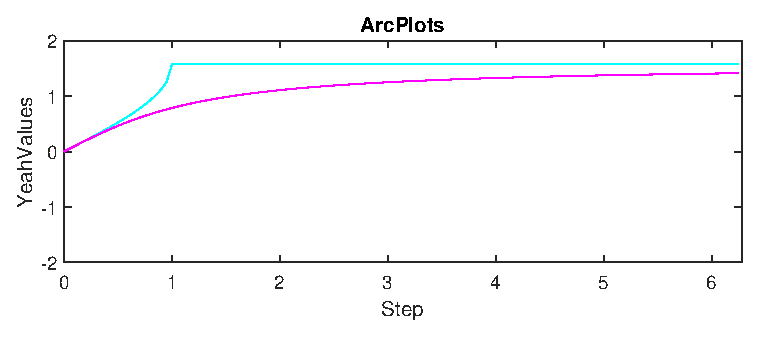
\includegraphics [width=4in]{Exercise_1_01.eps}


\subsection*{bode plots}

\begin{verbatim}
fprintf('\n%s\n', "d)")

K = [1, 1.5];
T = [1, 5, 10];
d = [0.5, 0.7, 1, 3];

for i = 1:2
    G1 = tf(K(i), [T(1), 1]);
    G2 = tf(K(i), [T(1)^2 2*d(1)*T(1) 1]);

    figure(1);
    bode(G1);grid on; hold on;
    title("GPT1 K dynamic");

    figure(2);
    bode(G2);grid on; hold on;
    title("GPT2 K dynamic");
end


for i = 1:3
    G1 = tf(K(1), [T(i), 1]);
    G2 = tf(K(1), [T(i)^2 2*d(1)*T(i) 1]);

    figure(3);
    bode(G1);grid on; hold on;
    title("GPT1 T dynamic");

    figure(4);
    bode(G2);grid on; hold on;
    title("GPT2 T dynamic");
end


for i = 1:4
    G = tf(K(1), [T(1)^2 2*d(i)*T(1) 1]);

    figure(5);
    bode(G);grid on; hold on;
    title("GPT2 d dynamic");
end
\end{verbatim}

        \color{lightgray} \begin{verbatim}
d)
\end{verbatim} \color{black}
    
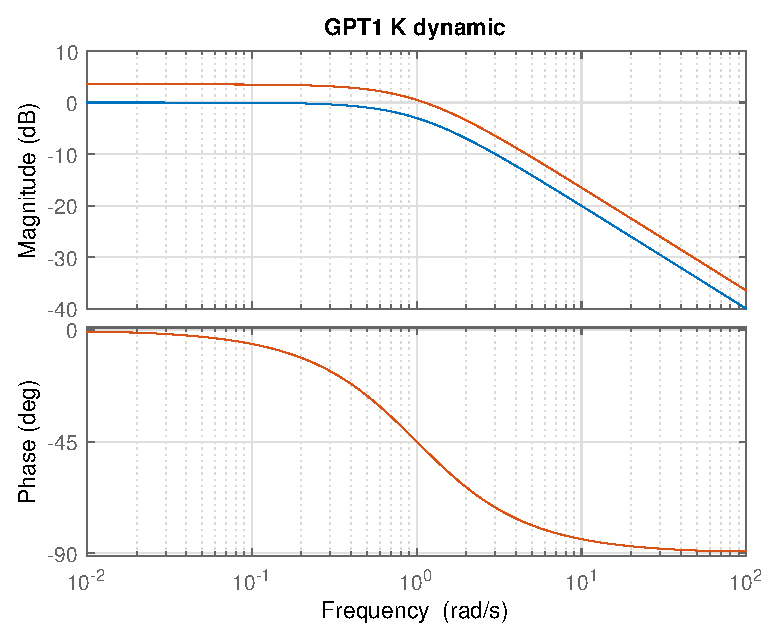
\includegraphics [width=4in]{Exercise_1_02.eps}

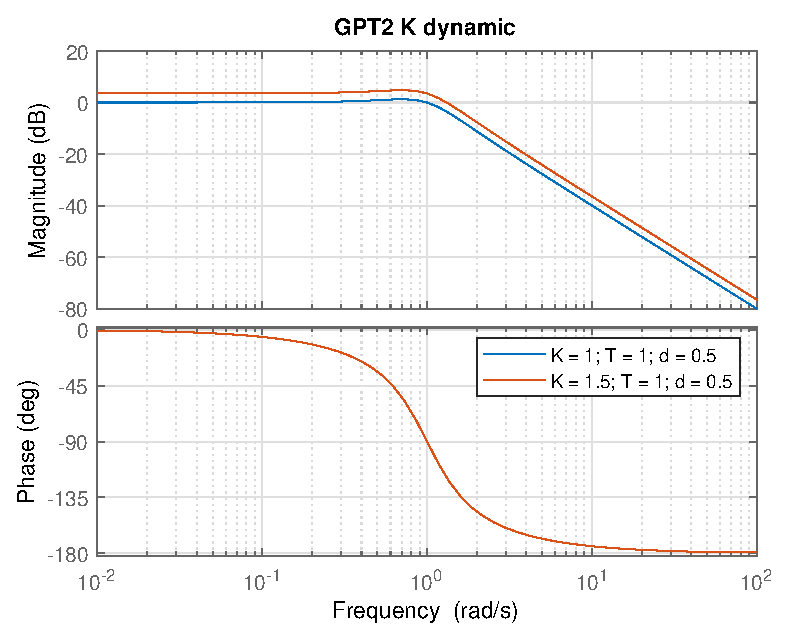
\includegraphics [width=4in]{Exercise_1_03.eps}

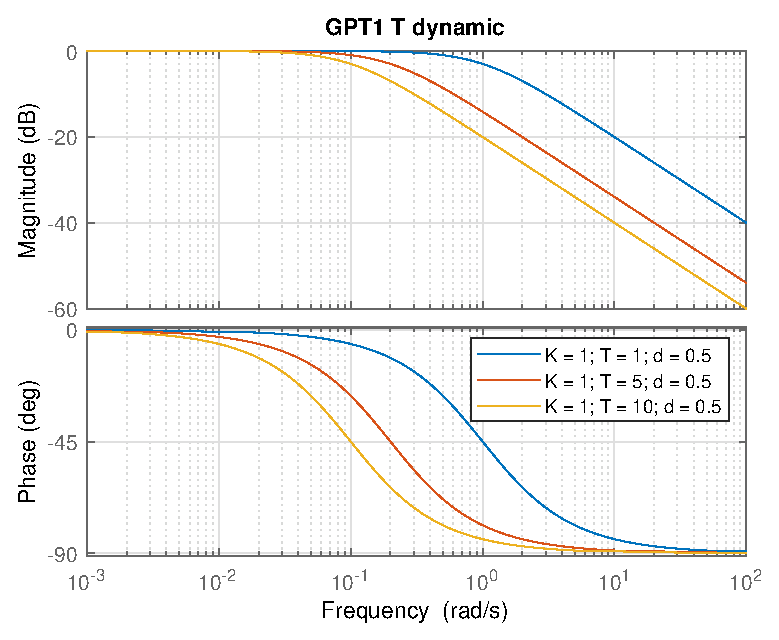
\includegraphics [width=4in]{Exercise_1_04.eps}

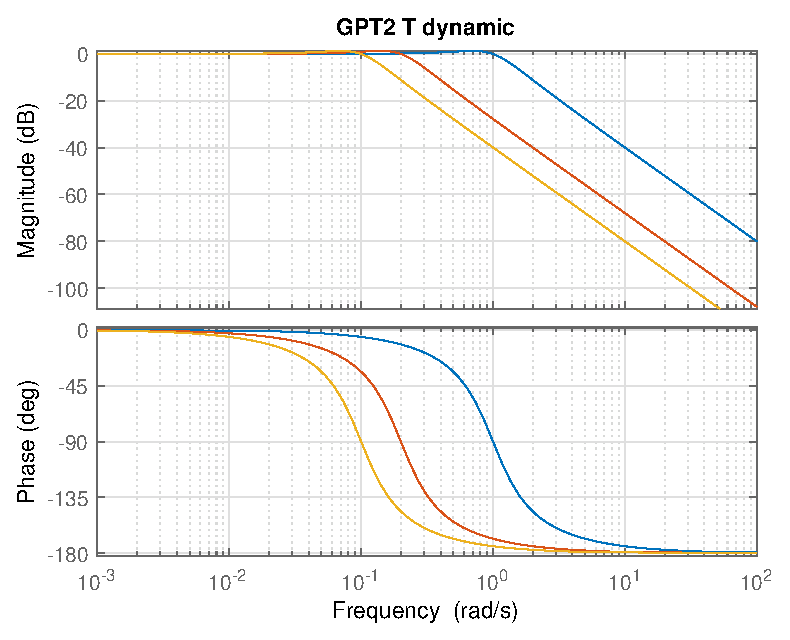
\includegraphics [width=4in]{Exercise_1_05.eps}

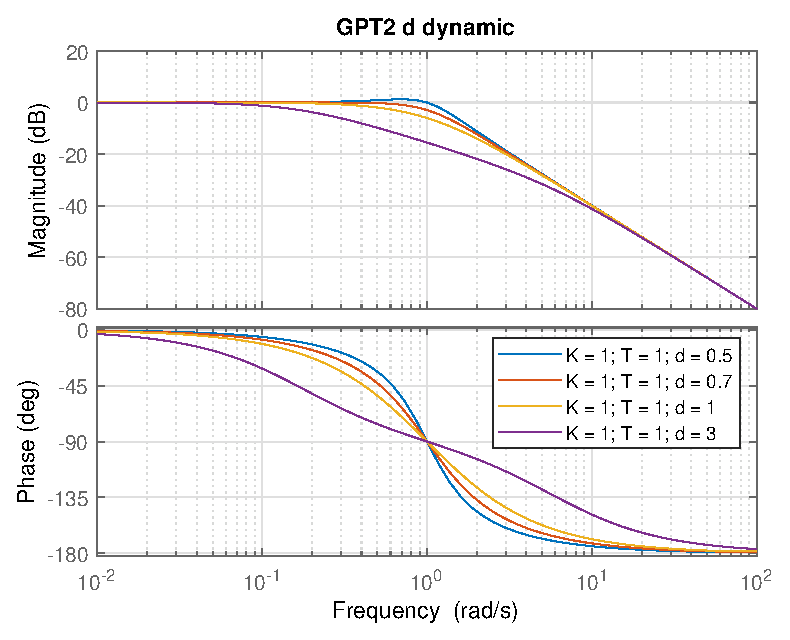
\includegraphics [width=4in]{Exercise_1_06.eps}


\subsection*{my bode}

\begin{verbatim}
steps = logspace(-2, 2, 1000) * 1i;

[mag, phase] = mybode(1, [2 1], 0, steps);

figure(1);
subplot(2, 1, 1);
semilogx(abs(steps), mag);
subplot(2, 1, 2);
semilogx(abs(steps), phase);


function [mag, phase] = mybode(a, b, Tt, w)
    if isempty(Tt)
        Tt = 0;
    end

    if isempty(w)
        w = logspace(-2, 2, 1000) * sqrt(-1);
    end

    g = polyval(a, w) ./ polyval(b, w) .* exp(-Tt * w);

    mag = 20 * log10(abs(g));
    phase = angle(g);
end
\end{verbatim}

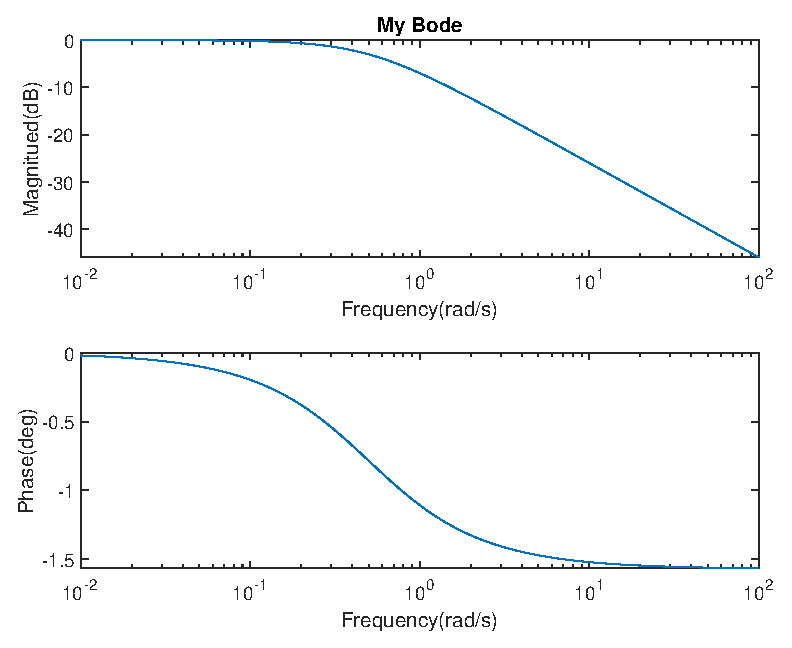
\includegraphics [width=4in]{Exercise_1_07.eps}



\end{document}
    
